
\chapter{Эвиденциальность: теоретические предпосылки исследования} \label{sec:ch1}

Настоящая глава посвящена эвиденциальности как типологической категории. В разделе \ref{sec:cat} изложено определение категории, лежащее на основе настоящей работы. Обсуждается семантическая зона эвиденциальности, способы выражения категории и ее коммуникативная функция. В разделе \ref{sec:small} мы сосредоточимся на "малых эвиденциальных системах", характерных для ареала, к которому относятся нахско-дагестанские языки. Особое внимание уделяется развитию форм косвенной засвидетельствованности из перфекта (раздел \ref{sec:pftyp}), поскольку именно эти формы представляют собой предмет настоящего исследования.

\section{Категория эвиденциальности} \label{sec:cat}

В нашем понимании \textsc{эвиденциальность} --- совокупность значений, обозначающих источник информации, лежащий в основе высказывания. Как отмечено в \citep[263--264]{boye2018}, понятие <<источник информации>> используется для определения данной категории в большинстве работ по эвиденциальности. Рисунок \ref{tab:evsem} суммирует как основные эвиденциальные контрасты, так и более дробную классификацию согласно разным типологическим обзорам \citep{willett1988, aikhenvald2004, plungian2010}. Схема построена по следующему принципу: отдельное место заслуживает каждое значение, которое связанно с указанием на источник информации и которое хотя бы в каком-то языке выражается отдельным показателем. Частные значения далее объединяются в более общие значения в том случае, если в каком-то языке они выражаются одним показателем. Категорию в целом обычно делят на прямую и непрямую эвиденциальность, что в русскоязычной литературе принято называть прямой и косвенной \textsc{засвидетельствованностью} \citep{kozintseva2007}. Предметом настоящей диссертации являются формы косвенной засвидетельствованности в видо-временной парадигме нахско-дагестанских языков. Эти формы могут иметь инферентивное или репортативное прочтение --- выбор той или другой интерпретации определяется контекстом (см. пример (\ref{ex:ali}) и обсуждение на ст. \pageref{p:context} во введении настоящей работы), а иногда форма имеет более общую функцию маркирования информации не из личного свидетельства.

% я не понял - чем отличается ситуация выбор той или иной интерпретации определяется контекстом, ... а ингда имеет более общую функцию маркирования информации не из личного свидетельства. Ведь двумя основными значениями непрямой засвидетельствованности как раз и являются репортатив и инферентив. А здесь как будет вы говорите о еще более широком значении, включающем что-то еще - а что еще? Надо это проговорить; либо убрать последнюю клаузу.

\begin{figure}[H]
\centering
\caption{Семантическая зона эвиденциальности}
\vspace{0.5cm}
\label{tab:evsem}
\begin{tabular}{lllll}
\textbf{Прямая засв.}    & \textgreater{} & личное участие         &                &                            \\
                         & \textgreater{} & чувственное восприятие & \textgreater{} & зрительное                 \\
                         &                &                        & \textgreater{} & слуховое                   \\
\textbf{Косвенная засв.} & \textgreater{} & умозаключение          & \textgreater{} & на основе очевидного       \\
\textbf{}                &                & (инферентив)           &                & результата или последствий \\
                         &                &                        &                & (инферентив)               \\
                         &                &                        & \textgreater{} & на основе имеющего знания  \\
                         &                &                        &                & (презумптив)               \\
                         & \textgreater{} & с чужих слов           & \textgreater{} & из третьих рук            \\
                         &                & (репортатив)           & \textgreater{} & из вторых рук             \\
                         &                &                        & \textgreater{} & из фольклора              
\end{tabular}
\end{figure}

В схеме не учтено значение \textbf{общего знания}. Во всех языках с категорией эвиденциальности есть тот или иной способ маркирования информации, полученной (выведенной) говорящим из общеизвестных фактов, которые сложно привязать к конкретному источнику (напр. <<мир круглый>>). В намбикварских языках есть специализированный показатель, указывающий на <<information that is known to the whole community, either because it is habitual, or because it is part of their mythological lore>> \citep[350]{eberhard2018}. В других языках общее знание маркируется либо формой прямой засвидетельствованности, либо формой презумптива. 
% опять не понял - чем отличается значение общего знания от формы презумптива? я всгда считал, что это одно и то же; если я не прав, лучше это проговорить, потому что читатель может быть не поймет. Также вопрос про то, что сказано ниже - вы говорите, что презумптив выражается общим прошедшим, а мне казалось, что некоторые из употреблений сочетаний с глаголом найти мы расценили как презумптивные (на грани с эпистемическими - где глагол найти в будущем времени - посомтрите.
Место этого значения в схеме остается не до конца ясным (см. обсуждение этой проблемы в \citep[35--38]{plungian2010} и \citep{verhees2019ev}). В нахско-дагестанских языках для таких случаев используется форма общего прошедшего, которая противопоставлена форме косвенной засвидетельствованности --- форма общего прошедшего может быть нейтральной в плане эвиденциальности (см., например, \citep[56]{forker2014} об эвиденциальности и общем знании в гинухском языке) или иметь оттенок прямой засвидетельствованности (см. \citep[274]{verhees2018} о рикванинском диалекте андийского языка). Подробнее о формах общего прошедшего и значение прямой засвидетельствованности в нахско-дагестанских языках см. раздел \ref{sec:direct}.
\par Мы также исключили из схемы значение \textbf{квотатива}. Хотя показатели чужой речи для настоящего исследования играют периферийную роль, это решение требует некоторого пояснения. Действительно, во многих работах о категории эвиденциальности (например в типологии А.Ю. Айхенвальд \citep{aikhenvald2004}), квотатив считается частью этой функциональной зоны. Во второй главе настоящей диссертации, помимо эвиденциальности в видо-временной парадигме, обсуждаются и другие грамматические средства выражения эвиденциальной семантики в нахско-дагестанских языках, поскольку они семантически частично пересекаются с видо-временными формами, конкурируют с ними и, тем самым, влияют на их употребление и грамматический статус. В нахско-дагестанских языках встречаются специализированные репортативы, специализированные квотативы, а также показатели, которые выполняют обе эти функции. Однако, как аргументируется ниже, на наш взгляд эти две функции, даже если они выражаются одним показателем, существенно различны. Только репортатив можно называть собственно <<эвиденциальным>> показателем, тогда как квотатив - это значение смежное, но все же отлично от собственно эвиденциальности. Чтобы понять, какие показатели чужой речи из нахско-дагестанских языков можно называть эвиденциальными показателями, нужно сначала понять, чем различаются репортативы и квотативы. 
\par Согласно А.Ю. Айхенвальд, репортатив обозначает информацию, полученную с чужих слов, тогда как квотатив указывает на цитату, т.е. содержит информацию, полученную от конкретного источника \textit{от конкретного источника} \citep[25]{aikhenvald2004}; оба значения она считает частью семантической зоны эвиденциальности. \color{black} Согласно \citep{holvoet2018}, <<эвиденциальными>> можно называть только такие квотативы, основной функцией которых является именно указание на источник информации, что в данном случае обозначает: вербальное сообщение от конкретного источника.
% я еще попробовал сформулировать так - квотатив указывают на цитату, и ТЕМ САМЫМ содержат информацию, полученную из вторых рук (но последнее не является их значением), а репортативы указываются ИМЕННО НА ТО, что информация получена из вторых рук (а получена она из конкретного источника или нет - это уже контекстно). Мне кажется, что так получается еще отчетливее?
На самом деле квотативы только косвенно указывают на источник, тогда как их функция --- маркирование речевого акта как цитаты. Это может быть не только цитирование чьих-то слов, но и цитирование мыслей, повтор собственных слов или воображаемое высказывание, приписанное определенному человеку, целой группе людей или недискретному интерлокутору, ср. пример (\ref{ex:mol}) с квотативной частицей \textit{мол}, где автор приписывает цитату своей предполагаемой аудитории.\footnote{Из: https://md-gazeta.ru/obshhestvo/4869.} Указание на какой-нибудь конкретный источник может и вовсе отсутствовать. Отметим, что примеры, приведенные в \citep{aikhenvald2004}, не противоречат определению квотативов как маркеры цитаты.

%не понял про "может и вовсе отсутствовать" - в примере про воображаемую аудиторию вроде бы так и есть? я бы сказал - Как показывает этот пример, эксплицитное указание на конкретный источник может отсутствовать, но источник при этом подразумеваться.

\lb{ex:mol}{\textit{Нужно развивать в себе рефлексивные умения --- давать оценку себе, своим действиям. Не обвинять молодежь, \textbf{мол}, она такая-сякая, а спросить у себя, в чем причина, почему же она <<такая>>.}}

На семантическх картах Л. Андерсона квотатив находится вне рамки семантической зоны эвиденциальности, аналогично другим выражениям, которые либо семантически близки к эвиденциальным выражениям, либо могут являються их диахроническим источником, но тем не менее не представляют часть концептуальной категории эвиденциальности. Такое представление функциональной зоны кажется нам наиболее удачным \citep[307]{anderson1986}.
\par Хотя типологические классификации эвиденциальности основаны в первую очередь на грамматических средствах ее выражения, большинство современных исследователей рассматривают эвиденциальность как \textbf{семантико-функциональную} категорию, значения которой можно выразить языковыми средствами разной природы. Среди них: грамматические показатели, лексические средства (например, вводные обороты, такие как <<видимо>>) и так называемые эвиденциальные \textsc{стратегии} --- формы или обороты, которые приобретают отличное от их основного значения эвиденциальное прочтение через контекстную импликатуры \citep[105--152]{aikhenvald2004}. \color{black}
В качестве примера эвиденциальной стратегии можно упомянуть некоторые модальные глаголы в германских языках, которые в определенных контекстах могут интерпретироваться как указание на то, что у говорящего есть некоторые косвенные основания для высказывания суждения. Ср. пример (\ref{ex:film}) из нидерландского языка, в котором используется глагол \textit{moeten} `должен', основной функцией которого является выражение деонтической модальности.\footnote{В данном случае автором диссертации был добавлен подстрочный перевод с глоссами на русском языке, потому что он в оригинале отсутстовал.} 

\lb{ex:film}{\gll De film \textbf{moet} uitstekend \textbf{zijn}.\\
{\Def} фильм должен.{\Prs} отличный быть.{\Inf} \\
\trans `The film \textbf{is said to be} excellent.’ \\
`\textbf{Говорят,} что фильм --- отличный.'\\ \footnotesize{\citep[74]{dehaan1999} \hfill нидерландский язык}}

В данном случае эвиденциальное прочтение возникает из контекста. Если человек утверждает, что <<фильм должен быть отличным>>, подразумевается, что его убеждение на чём-то основано. При этом маловероятно, чтобы это было прямым знанием - в этом случае он скорее сказал бы, что <<фильм --- отличный [я его видел]>>. Такая интерпретация употребления деонтической формы достаточно естественна, но языки различаются между собой тем, насколько та или иная эвиденциальная интерпретация приемлема и распространена. В нидерландском языке пример (\ref{ex:film}) однозначно интерпретируется \textsc{репортативно} (т.е. как передача информации с чужих слов).\footnote{В устной речи интонация может влиять на интерпретацию --- если фразовое ударение на модальном глаголе, доступна лишь деонтическая интерпретация.} Напротив, аналогичный пример с английским глаголом \textit{must} скорее всего понимается как умозаключение говорящего (например, ему понравились другие фильмы того же режиссера) и передает оттенок уверенности со стороны говорящего \citep[81]{auweraplungian1998}. В нидерландском языке такие оттенки отсутствуют. Эвиденциальное значение нидерландского \textit{moeten} --- периферийное явление наряду с другими значениями, описанными в диахронической перспективе в \citep{olbertzhonselaar2017}.\footnote{Стоит отметить, что, насколько мы знаем, не существует корпусного исследования использования данного глагола как показателя эвиденциальности; неизвестно, возникает ли оно в равной степени часто в разных конструкциях с этим глаголом. Для английского must, например, известно, что эпистемическое значение более частотно в определенных синтаксических контекстах \citep{dehaan2012must}. Глагол \textit{moeten} как показатель эвиденциальности обсуждается в основном в работах \citep{dehaan1997} и \citep{dehaan1999}, где неизменно приводится один и тот же пример, цитируемый нами выше (\ref{ex:film}). Следовательно, когда мы говорим, что это <<периферийное явление>>, мы опираемся не на результаты систематического исследования (хотя отсутствие упоминания эвиденциального значения в подробном анализе \citep{olbertzhonselaar2017} можно считать показательным), а на собственную языковую интуицию (нидерландский является родным для автора настоящего исследования). Кажется по крайней мере, что нидерландский \textit{moeten} более характерен для устной речи и не является аналогом немецкого \textit{sollen}, который широко употребляется в письменной речи, см. например \citep{vanderbiesen2018}.} При этом эвиденциальное прочтение можно "отменить", добавив, например, <<иначе я потребую возврата денег>> (т.е. <<фильм должен быть отличным>> в таком случае значит <<если фильм не отличный, (то я потребую возврата денег)>>). Это подтверждает, что форма не является примером грамматического выражения эвиденциальности.
\par Эвиденциальное значение нахско-дагестанских форм косвенной засвидетельствованности также возникает из импликатуры (подробнее об этом процессе в разделе \ref{sec:pftyp}), но на интерпретацию форм влияет не только внелингвистический контекст, но и структура формы, конструкции или предложения. В одних случаях эвиденциальное прочтение возможно, но при этом всегда возможно отменить его, а в других случаях другая интерпретация невозможна в принципе. \color{black} Значение Перфекта в аштынском даргинском, например, может быть только эвиденциальным, когда форма образована от имперфективной основы глагола, как в примере (\ref{ex:selsov}). Аналогичная форма, образованная от перфективной основы, может быть перфектной или эвиденциальной \citep[202--204]{belyaev2012}.

\lb{ex:selsov}{\gll ucːi-l kaʁaj-ti \textbf{ka-d-iːž-ipːi} selsawet-li \\
брат-{\Erg} письмо-{\Pl} down-{\Npl}-писать.{\Ipfv}-{\Pf} сельсовет-{\In}\\
\trans `Мой брат \textbf{писал} письма в сельсовет.’ \\
Контекст: говорящий разговаривал с братом по телефону, т. е. не видел его\\
\footnotesize{\pgcitep{belyaev2012}{202}} \hfill даргинский: аштынский}

Пример (\ref{ex:sit}) с перфективной глагольной формой из ицаринского даргинского имеет две возможных интерпретации: 1) \textsc{результативная} (говорящий сел и сейчас сидит) или 2) \textsc{эвиденциальная} (говорящий по какой-то причине не был осознанным свидетелем собственного действия и делает вывод о том, как он оказался в таком положении).\footnote{Результативное значение в примере (\ref{ex:sit}) очень похоже на собственно перфектное значение и часто считается членом семейства перфектных значений, но оно представляет более ранний этап грамматикализации --- об отношениях между результативом и перфектом вообще см. в разделе \ref{sec:pftyp}, а конкретно в нахско-дагестанских языках в разделе \ref{sec:perf}.}

\lb{ex:sit}{\gll kiž-ib-li-da\\
sit\_down.{\Pfv}-{\Pst}-{\Cvb}-{\First}{\Sg}\\
\trans 1. `I am sitting.' / `Я сижу.'\\
2. `[It appears] I sat down.' / `[Оказывается, что] я сел.'
\footnotesize{\\\citep[450]{tatevosov2001} \hfill даргинский: ицаринский}}

Разного рода стратегии и их эвиденциальное прочтение в конкретных языках демонстрируют разную степень грамматикализованности и часто служат диахроническим источником для грамматических показателей эвиденциальности \citep[267--280]{aikhenvald2004}. Поскольку одна из целей настоящего исследования --- попытка оценить статус категории эвиденциальности в грамматике нахско-дагестанских языках, для нас важно различить разные виды стратегии с точки зрения наличия контекстов, в которых эвиденциальное прочтение является прочтением по умолчанию. Соответственно, мы различаем следующие четыре способа выражения эвиденциальности:\footnote{Под словом <<единицы>> имеются в виду любые языковые средства выражения эвиденциальной семантики: лексические единицы, специализированные морфемы, конструкции и т.д.}

\begin{enumerate}
    \item \textbf{Единицы с неотъемлемым эвиденциальным значением}\footnote{Неотъемлемым значением мы считаем значение, которое по умолчанию выражается определенной формой в немаркированном контексте.}\\
% по больщому счету, не очень ясно, что такое "немаркированный контекст" - но давайте оставим как есть
    Маркирование источника информации при этом \textit{обязательно}\\
    (грамматические способы)
    \item \textbf{Единицы с неотъемлемым эвиденциальным значением}\\
    Маркирование источника информации при этом \textit{необязательно}\\
    (грамматические и лексические способы)
    \item \textbf{Единицы с эвиденциальным значением, которое зависит от составляющих конструкций или предложения}\\
% я бы написал просто "которое появляется в определенной конструкции" - что такое "зависеть от составляющих конструкций и предложения" - это претендует на как бы большую точность, но на самом деле менее ясно. 
    (грамматические способы и эвиденциальные стратегии)
    \item \textbf{Единицы с эвиденциальным значением, которое зависит от дискурсивного контекста}\\
% я бы написал просто "которое появляется в определенном дискурсивном контексте" - непонятно, что значит "значение зависит от контекста"
    (эвиденциальные стратегии)
\end{enumerate}

% мне на самом деле не очень нравится эта классификация - неясно, что имеется в виду по сути под грамматическими  и лексическими средствами и стратегиями. например, ваш пример голландский - его хочется считать лексическим, но он появляется в определенных контекстах, поэтому он стратегия. кажется, что различение между стратегиями, с одной стороны, и морфологическими, лексическими и конструкционными средствами, с другой - это две независимые классификации. И еще я бы называл ваши грамматические - морфологическими, а грамматичность если как-то бы определял, то по степени обязательности. Если обязательное эквиполентное противопоставление (индиректив vs директив) грамматическое; только индиректив, но обязательный - полу- или слабограмматическое; если ни то, ни друго необязательно - неграмматическое. А морфология, лексика или конструкция - это ортогональная классификация. Но я не уверен, что мы сможем сейчас это все обсудить и изменить так, чтобы обоих устроило.

В \textbf{первую категорию} входят только строго грамматические показатели эвиденциальности.\footnote{В настоящей работе мы называем такие формы <<эвиденциальными показателями>>. Этот термин мы применяем только к таким формам, а формы промежуточного статуса называем формами или выражениями с эвиденциальным значением, имплицируя, что это не их единственное значение.} % Сюда добавить про то, что можно и использовать слово "эвиденциалы" как делают ММ и некоторые другие.
% снова - я не понимаю этого рассуждения. они являются строго грамматическими показателями по другим критериям (тогда по каким?), или вы так ОПРЕДЕЛЯЕТЕ строго грамматические показатели. вроде бы не последнее, потому что грамматические есть и во второй категории. здесь основания классификации неясны. И ниже тоже неясно; иногда начинается казаться, что грамматические показатели - для вас просто морфологические показатели - это так? если это так, то я бы так и сказал, и это сняло бы многие проблемы.
Внутри \textbf{второй категории} можно при необходимости различать лексические и грамматические единицы. Лексические выражения непосредственно (самим своим лексическим значением) указывают на (вид) источника информации; таким образом, обороты типа <<говорят>> отличаются от факультативных репортативных частиц непрозрачной этимологии. В ботлихском языке нахско-дагестанской семьи, например, имеется репортативная частица \textit{χʷata} (см. пример (\ref{ex:cow}) ниже). Если во многих нахско-дагестанских языках такого рода частицы явно восходят к глаголом говорения (см. раздел \ref{sec:clitics}), происхождение ботлихской частицы остается неясным. 
%хотя я в приницпе тут согласен, но мне кажется тут имеет место существенное упрощение действительности. есть масса промежуточных случаев, когда происхождение ясно лингвисту, но не носителю (в арчинском). я бы либо представлял это в качестве шкалы, либо говорил, на худой конец, что есть регулярные формы лексических единиц, конвенционализированные в фукнции передачи эвиденциальных значений; а есть нерегулярные формы или частицы вообще неизвестного поисхождения. Аааа, ой, у вас ниже про это! извините. на всякий случай оставляю свои соображение, to be sure we re on the same wave.

\lb{ex:cow}{\gll zini hiƛ’a	b-ukː-u=\textbf{χʷata} \\ 
корова вниз	{\N}-упасть-{\Aor}={\Rep} \\
\trans `Корова упала, \textbf{говорят}.' \\ \footnotesize{[полевая работа 2018-го года] \hfill ботлихский язык}}

Частица в примере (\ref{ex:cow}) указывает на то, что информация, передаваемая основной пропозицией (<<корова упала>>), получена с чужих слов. При этом употребление данной частицы в таких случаях необязательно. Однако единицы не всегда можно однозначно охарактеризовать как этимологически прозрачные или непрозрачные (ср., например, русскую частицу <<мол>>). В таких случаях помогает функциональный подход к их разграничению, предложенный в \citep{boyeharder2012}; согласно этому подходу, грамматические единицы передают дискурсивно вторичную информацию, тогда как лексические единицы носят основную смысловую нагрузку высказывания. 

% так более понятно?
% смысл понятен, но мне не нравится формулировка, и не вполне точно, на мой взгляд, передают цитату ниже - важен компонент "потенциально", потому что лексические единицы МОГУТ не нести дискурсивно prominent информации, но могут и нести, а грамматические - как бы в принципе не могут (но сам не решился перифразировать чтобы не переврать):
% согласно этому подходу, грамматические единицы всегда передают вспомогательную, дискурсивно вторичную информацию, в то время как лексические единицы могут (хотя и не обязаны) нести основную смысловую нагрузку высказывания  

\begin{displayquote}
<<[...] grammar is constituted by expressions that by linguistic convention are ancillary and as such discursively secondary in relation to other expressions [...]. Conversely, lexical expressions are by linguistic convention potentially primary in terms of discourse prominence. The concept of discourse prominence is understood in terms of a core idea that we regard as essentially uncontroversial: in entertaining complex mental content, there is always a priority dimension involved, so that some parts of the content are more highly prioritized than others>>\\
\citep[2]{boyeharder2012}
\end{displayquote}

На наш взгляд, такое определение позволяет принимать более последовательные решения, хотя результат может противоречить традиционным представлениям о лексиконе и синтаксисе. Как отмечено в \citep[3]{cornillie2015}, сентенциальные наречия с эвиденциальной семантикой (в отличие от матричных предикатов с той же семантикой) оказываются грамматическими показателями, несмотря на то, что и те, и другие прямо указывают на (вид) источника информации. Впрочем, для настоящего исследования различие между лексическими и грамматическими средствами не принципиально.
\par \textbf{Третья} и \textbf{четвертая категории} пересекаются в том смысле, что одна и та же форма может попадать в обе категории: она может иметь контексты употребления, в которых эвиденциальное значение является для нее единственным или значением по умолчанию, тогда как в других контекстах оно может быть обусловлено дискурсивным контекстом, как, например, в случае аштынского перфекта, образуемого от основы имперфектива (эвиденциальное прочтение по умолчанию) или перфектива (эвиденциальное значение может наводиться дискурсивно). 
% внимание - я не понял, что тут было сказано, так как был какой-то неправильный синтаксис - попробовал исправить, но проверьте смысл
Наша классификация позволяет таким образом разложить одну форму на разные конструкции с разного типа эвиденциальным значением. Это позволяет более отчетливо различить разного рода контексты употребления и их роль в интерпретации формы.
\par Помимо семантики и способа выражения, категорию эвиденциальности можно рассматривать с точки зрения ее \textbf{коммуникативной функции}: эвиденциальные показатели устанавливают связь между моментом речи и его участниками и событием, о котором идет речь, просредством некоторого промежуточного события, в результате которого говорящий получил сообщаемую информацию. Их значение соответственно зависит от речевой ситуации и ее участников. 
% я не понял смысл последнего предлождения, но зато оно кажется не мешает и не помогает понимать следующее (смайлик), так что я бы снял просто его.
С этой точки зрения, эвиденциальные показатели --- \textsc{эгоцентричные} элементы: они по умолчанию интерпретируются как указывающие на источник информации говорящего.\footnote{Слово <<эгоцентричный>> мы здесь используем согласно \citep[258--284]{paducheva2010}, хотя стоит отметить, что Е.В. Падучева в своей работе не обсуждает эвиденциальность, что возможно связано с тем, что эвиденциальность как грамматическая категория нехарактерна для русского языка.} Исключение могут составлять вопросительные предложения: в шайенском языке алгонкинской семьи один и тот же (репортативный) показатель интерпретируется в утвердительном предложении как относящийся к говорящему (\ref{ex:chey1}), а в вопростиельном --- к адресату (\ref{ex:chey2}).

\lb{ex:chey1}{\gll ná-hó’tȧhevá-\textbf{mȧse}.\\
	{\First}-win-{\Rep}.{\First}{\Sg}\\
    \trans `I won, \textit{I hear}.’\\
    `[Я слышал, что] я выиграл.'\\
    \footnotesize{\citep[45--46]{murray2017} \hfill шайенский язык}}
    
\lb{ex:chey2}{\gll \textbf{mó}=ná-hó’tȧhevá-\textbf{mȧse?}\\
    {\Q}={\First}-win-{\Rep}.{\First}{\Sg}\\
    \trans `\textit{Given what you heard,} did I win?’\\
    `[Что ты слышал ---] я выиграл?'\\
    \footnotesize{\citep[45--46]{murray2017} \hfill шайенский язык}}

Впрочем, такого рода <<переключение>> в вопросах (interrogative flip) происходит не во всех языках, см. \citep[43--50]{murray2017}. Кроме того, в нарративном контексте показатели эвиденциальности могут указывать на источник информации не говорящего, а персонажа, см. раздел \ref{sec:intro3} настоящей работы.
% здорово, интересно! при этом этот персонаж не является вложенным говорящим, да? а просто кем-то, про кого идет речь? (потому что если он вложенный говорящий - это неинтересно, это просто смена перспективы в цитате; а тут читатель подумает что-то вроде того, что подумал я).
\par В формальной литературе такое <<реляционное>> определение эвиденциальности достаточно распространено, см. обзор в \citep{speas2018}. В своей основополагающей работе о глагольных категориях Р.О. Якобсон классифицировал эвиденциальность как <<шифтерную>> категорию, наряду со временем и личным дейксисом \citep{jakobson1957}. Тем не менее, в функционально-типологической литературе такой взгляд на эвиденциальность оказался в фокусе теоретических дискуссий только в последние годы, например в работе Х. Бергквиста, который рассматривает эвиденциальность как дейктическую категорию \citep{bergqvist2018}, опираясь в том числе на модель реляционного дейксиса В. Хенкса \citep[12]{hanks2009}. Согласно Бергквисту, эвиденциальные показатели не просто устанавливают связь между событиями, но и определяют дистанцию между ними, которая может быть измерена степенью опосредованности доступа к информации. Грубо говоря, прямая засвидетельствованность --- своего рода ближний дейксис, а косвенная засвидетельствованность --- более дальний \citep[21--23]{bergqvist2018}. Возможно наиболее уместный термин для таких подходов в совокупности будет \textsc{индексальный}, как предложено в \citep{hanks2014}.\footnote{См. также дискуссию о проблемах, связанных с использованием термина <<дейктический>> в \citep[265--267]{boye2018}.}

\begin{displayquote}
<<Evidential marking is a species of indexicality in which the evidential form indexes the relation between the Speaker, the object or event spoken about and the linguistic act of producing the `evidential utterance.’ It therefore calls for three overlapping lines of research: grammar, semantics, and pragmatics.>>\\
\citep[169]{hanks2014}
\end{displayquote}

Из индексальной природы эвиденциальности следует, в частности, что категория передает фоновую информацию: 
% если это интерпретация приведенной цитаты, мне не кажется, что она правильная - в цитате просто сказано, что эвиденциальность передает вторичную информацию, не сказано, что это потому, что она индексальная. И действительно, индексальные элементы вполне могут быть лексическими по вашему данному выше определению и мочь нести фокус, ассерцию высказывания - личные, указательные местоимения. Я бы переформулировал типа:
% Согласно Андерсону (\citep{anderson1986}), эвиденциальная категория передает фоновую информацию:
<<Evidentials are not themselves the main predication of the clause, but are rather a specification added to a factual claim about something else>> \citep[274]{anderson1986}. Поэтому значение эвиденциальных показателей, как правило, не поддается отрицанию, потому что в центре внимания является содержание основной пропозиции, тогда как источник сведений о нем не находится в фокусе внимания (\textit{not at issue}), ср. \citep[28--30]{murray2017}. Вклад эвиденциальных показателей в семантику высказывания в целом можно рассматривать как своего рода \textsc{метапропозицию}, которой пропозиция подчинена \citep[151]{evans2018}. % Мне кажется, что вроде стало ясно что я в основном опираюсь на функциональную литературу, а не на формальную. Я не думаю что стоит еще эксплицитно говорить, что я дальше ее не принимаю во внимание.
% мне показалось, что Диана говорила о другом - не о том, что вы опираетесь на функциональную, а не на формальную литературу (это и так было ясно), а о том, что в вашем тексте не отражено, что вы вообще знаете о ее существовании. Вот это стоило бы где-то отразить - необязательно именно здесь, но где-то.
\par Преимущество индексальных подходов заключается в том, что они позволяют более адекватно анализировать функционирование эвиденциальности в речи с учетом речевой ситуации и по сравнению с другими индексальными категориями, т.е. временем и лицом. Это помогает объяснить неожиданные на первый взгляд смены форм и переключения перспективы, что оказывается суещственным для эмпирического исследования категории эвиденциальности в третьей главе настоящей работы.

\section{Малые эвиденциальные системы} \label{sec:small}

Как уже было отмечено во введении, в определенных ареалах системы выражения эвиденциальных значений демонстрируют определенные сходства. Наиболее сложные системы представлены в языках коренного населения Америк, как например в туканских языках Южной Америки, которые различают от трех до шести разных источников информации обязательными глагольными аффиксами, кумулятивно выражающими эвиденциальность, время/вид и согласование по роду/лицу \citep{stenzelgomez2018}. Различаются в том числе зрительное и другие типы восприятия (т.е. говорящий не видел события, но услышал, например, предполагающий событие звук или почувствовал соответствующий запах или прикосновение, ср. пример (\ref{ex:gnat}) из языка тукано), логический вывод на основе очевидных последствий (инферентив) или общепринятого знания (презумптив), а также знание, полученное с чужих слов (репортатив).
% Кстати, не точнее ли будет сказать - Южной Америки? это и изящнее, и может быть точнее? или в северной америке тоже богатые системы?

\lb{ex:gnat}{\gll \textasciitilde{}ahú\textasciitilde{}pea 	\textasciitilde{}badî-de \textbf{\textasciitilde{}du’dî-\textasciitilde{}da’} \textbf{weé-sa-\textasciitilde{}ba} \\ 
biting.gnats {\First}{\Pl}.{\Incl}-{\Obj} bite-{\Ss} do-{\Nvis}-{\Third}{\An}.{\Pl} \\
\trans `Gnats \textbf{are biting} us! (the insects are too small to see, but the bites can be felt.'\\
`Мошки \textbf{кусают} нас! (насекомых не видно, потому что они слишком маленькие,\\ но их укусы чувствуются)' \\ \footnotesize{\citep[131]{ramirez1997}\footnote{По \citep[367]{stenzelgomez2018}} \hfill язык тукано}}

Ареал нахско-дагестанских языков находится в центре так называемого \textsc{эвиденциального пояса} (также: <<Эвиденциальный пояс старого света>> \citep[63]{sumbatova1999}), охватывающего часть Восточной Европы, Кавказ, Среднюю и Южную Азии и Сибирь.\footnote{Нам не удалось выяснить, кто первым употребил термин <<эвиденциальный пояс>> --- он часто употребляется, например, в \citep[290]{aikhenvald2004}, \citep[19]{plungian2010} и во многих других работах, но, как правило, без ссылки на других авторов.} По типологии Айхенвальд <<малые>> системы (обозначены буквой А в \citep{aikhenvald2004}), выражают только одно или два значения, среди них: прямая vs. косвенная засвидетельствованность (A1), косвенная засвидетельствованность (A2), репортатив (A3), значительно реже: чувственное восприятие и репортатив (A4), слуховое восприятие (A5). В языках эвиденциального пояса представлены в основном системы типа A1, A2, A3. При этом во многих языках сосуществуют несколько независимых систем, так что показатели могут быть <<разбросаны>> по грамматике: так называемое scattered coding \citep[8--11]{aikhenvald2003}. На Кавказе часто сосуществует эвиденциальность в видо-временной парадигме, осуществляющая базовый контраст прямой и косвенной засвидетельствованности (или маркирующей только косвенную засвидетельствованность по контрасту с нейтральной формой), и специализированная частица для репортатива или (реже) инферентива. 
% именно репортатива? не квотатива? или про квотатив вы здесь уже не говорите вообще? может быть, имеет смысл тогда либо напомнить, что квотатив уже не рассматривается; либо же сказать, что здесь речь идет о квотативно-репортативных частицах. 
\par Эвиденциальность внутри глагольной парадигмы часто восходит к перфектной форме глагола, которая приобретает оттенок косвенной засвидетельствованности (об этом подробнее в разделе \ref{sec:pftyp}). В результате грамматикализации перфектной формы противопоставленная ей менее маркированная форма прошедшего времени (Общее Прошедшее, Претерит, Аорист или Простое Прошедшее) может по контрасту переосмысляться как форма прямой засвидетельствованности. С другой стороны, частицы часто происходят от глаголов речи в роли матричного предиката или глаголов типа `казаться' (см. раздел \ref{sec:clitics} для примеров из нахско-дагестанских языков).
\par Вероятным источником для распространения эвиденциальности в пределах Пояса считаются тюркские языки, поскольку в этих языках древность категории подтверждается ее наличием в старых памятниках письменности, ср. \citep[273]{erdal2004}, а также потому, что она до какой-то степени присутствует во всех современных языках семьи \citep[510--511]{johanson2018}.
% вот этот абзац и следующий надо переписать с учетом того, что нам написала Анна Владимировна
При этом тюркские языки географически разбросаны почти по всей обсуждаемой территории, включая и Восточный Кавказ. Гипотеза о том, что появление эвиденциальности в глагольной системе связано с контактами с тюркскими языками, специалистами оценивается как возможная по крайней мере для грузинского \citep[297--298]{boeder2000} и восточноармянского \citep[415]{kozintseva2000} языков. Для этих двух языков имеются древние памятники письменности, которые помогают проследить появление того или иного употребления, учитывая при этом историю контакта с тюркскими народами (хотя насколько мы знаем, точная хронология этих процессов пока не исследовалась). С другой стороны, эвиденциальные формы глагола в западнокавказских языках оцениваются В.А. Чирикбой как предшествующие усилению контактов с местными тюркоязычными народами \citep[265--267]{chirikba2003}.
\par Для нахско-дагестанских языков пока не была предпринята попытка оценка вероятности данной гипотезы, кроме обсуждения ареального распределения эвиденциальности внутри семьи в \citep{verhees2018pstgu}. В разделе \ref{sec:dagturk} настоящей работы мы обсудим гипотезу о развитии категории эвиденциальности в нахско-дагестанских языках под влиянием тюркских языков на фоне представлений о языковом контакте, принимая во внимание не только то, как устроены эвиденциальные системы в исследуемых языках, но и географическое распределение свойств этих систем и языков в пределах ареала.

\subsection{Типология перфекта и косвенной засвидетельствованности} \label{sec:pftyp}

\color{black}
Перфект --- форма глагола. Перфект часто рассматривается как вид, хотя на самом деле его семантика сочетает вид со временем, ср. \citep[6]{comrie1976}. Сам термин <<перфект>> часто отождествляется с семантикой так называемой <<текущей релевантности>>: совершенное в прошлом действие определенным образом релевантно для момента речи \citep[24--25]{comrie1985}. Текущая релевантность (дальше ТР) представляет собой обобщение четырех более частных значений, перечисленных ниже и проиллюстрированных на примерах употребления английского Перфекта (present perfect).\footnote{Здесь мы опираемся на обзорную статью Е.-М. Ритз \citep[882--884]{ritz2012}, те же значения перечисляются, например, в \citep{comrie1976} и \citep{mccawley1971}.}

\begin{enumerate}
    \item \textbf{Результативный перфект (perfect of result / stative perfect)}\\
    Совершенное в прошлом действие с результатом или последствиями \\ в настоящем.\\
    John has gone.\\
    `Джон ушел (и его сейчас нет).'
    \item \textbf{Континуатив (continuative / universal perfect)}\\
    Действие было совершено за определенный промежуток времени в \\ прошлом, и до сих пор продолжается.\\
    John has worked here for 20 years.\\
    `Джон работал здесь 20 лет (и он до сих пор здесь работает).'
    \item \textbf{Недавнее прошедшее (perfect of recent past / <<hot news>> perfect)}\\
    Действие совершилось только что, и его завершение является \\ (неожиданной) новостью для говорящего, адресата или обоих.\\
    John has just resigned.\\
    `Джон (только что) подал в отставку.'
    \item \textbf{Экспериентив (experiential / existential perfect)}\\
    Некоторое действие совершилось по крайней мере один раз в прошлом.\\
	John has been to Japan.\\
	`Джон бывал в Японии (он имеет такой опыт).'
\end{enumerate}
 
Перфекты могут иметь разные диахронические источники, но в настоящей работе мы сосредоточимся на перфекте, восходящем к результативным конструкциям. Именно такое развитие характерно в целом для Евразии и, в частности, для нахско-дагестанских языков. Все перфектоподобные формы, рассматриваемые нами в разделе \ref{sec:perf}, с большой вероятностью имеют результативное происхождение, что подтверждается наличием значения узкого результатива у многих из них и, косвенно, высокой степенью формального сходства между формами разных языков. \textsc{Результатив} в узком понимании (т.е. результативная конструкция) образует одновалентный предикат, обозначающий совершенное в прошлом действие \textit{с результирующим состоянием в настоящем} \citep[10]{plungian2016}. Это значение обычно складывается непосредственно из составляющих конструкции: нефинитная форма с семантикой прошедшего времени или совершенного вида в сочетании со вспомогательным глаголом в настоящем времени. Результативы типично ограничиваются предельными предикатами, хотя есть некоторые исключения \citep[25]{nedjalkov1983}. 
\par По \citep{bybee1994}, результатив может развиваться в сторону перфекта текущей релевантности (у Байби и др. anterior) и далее в перфективное или простое прошедшее, как это произошло, например, в романских языках. На стадии перфекта / ТР отдельные значения характеризуются разной степенью грамматикализованности, что проявляется в их сочетаемости с разного рода предикатами. Результативный перфект, аналогично узкому результативу, указывает на совершенное в прошлом действие, но с \textit{результатом} в настоящем; он он не ограничивается предельными предикатами и необязательно обозначает некоторое очевидное результирующее состояние. В отличие от результатива, результативный перфект допускает присутствие действующего субъекта и не сочетается со словом <<еще>>, см. подробнее об этом в разделе \ref{sec:perf}. Континуативное значение возникает при сочетании с непредельными глаголами. В целом перфект как бы <<инвертирует>> семантику исходного предиката: из предельных предикатов он образовует дуративное состояние, а из непредельных предикатов --- завершенное действие. Экспериентив считается более продвинутым уровнем грамматикализации перфекта \citep[379]{lindstedt2000}.

% Ниже у ТА был комментарий по поводу "конвенционализация разговорной импликатуры" - не понравилось "разговорная", но дальше он оставил как есть. Помню, что у нас с вами тоже была дискуссая об этим термине - разве нет нормального русского перевода понятия conversational implicature. На мой взгляд это все-таки не совсем то, что просто импликатура, ведь бывают разного рода имликатуры.
% разговорная не очень хорошо, мне кажется. я бы говорил про дискурсивную (как выше) или контекстную или прагматическую импликатору - разговорный по-русски значит в первую очередь или исклбчительно colloquial. 

\par Развитие значения косвенной засвидетельствованности проходит иным образом, через конвенционализацию импликатуры. Согласно Левинсону, разговорная импликатура представляет собой имплицитное значение выражения, подразумеваемое участниками момента речи. 
% ну вот да, разговорная - странно. и еще не может быть участников момента речи - участниками речевого акта в момент речи? частные я бы назвал окказиональными.
Имплицитные значения бывают \textsc{частными}, т.е. случайными, обусловленными конкретным контекстом, или \textsc{общими} --- более менее стандартные презумпции, вызываемые семантикой самой единицы, ср. адаптированный пример (\ref{ex:party}) из \citep[16]{levinson2000}.

\lb{ex:party}{\textit{Some} guests \textit{are leaving} the party.\\
Общая импликатура: некоторые остаются, не все уходят.\\
Частная импликатура: наверно уже поздно.}
% у вас здесь общая, а ниже в абзаце - обобщенная. это одно и то же? я бы сказал "через конвенционализацию обобщенной импликатуры"
При частом употреблении имплицитное значение может становиться конвенциональным, что в свою очередь может вести к (частичному) переосмыслению самого языкового выражения \citep[81--82]{hoppertraugott2003}. Известным примером является развитие конструкции \textit{be going to} в английском языке. Исходно конструкция с глаголом движения \textit{go} указывала на движение в пространстве, но через обобщенную импликатуру она превратилась в показатель будущего времени. Конструкция с модальным глаголом в нидерландском языке, представленная нами в примере (\ref{ex:film}), в этом смысле находится на полпути. Репортативная интерпретация достаточно распространена, и глагол употребляется для того, чтобы вызвать такую интерпретацию, но модальная интерпретация во всех контекстах остается возможной. По сравнению с ней, английская конструкция \textit{be going to} за счет нового значения распространилась на новые контексты, где пространственная интерпретация невозможна, например в сочетании с инфинитивом, ср. пример (\ref{ex:army}) ниже, по \citep[263]{levinson2000}, который можно перефразировать как \textit{He is going to serve in the army} (`Он будет служить в армии'). 
% я честно говоря не понял почему пространственная интерпретация с инфинитивом невозможна - он идет курить - это у Левинсона так? Если у ЛЕвинсона - то ладно, пусть будет.
\lb{ex:army}{1. He \textit{is going} to the army. (`Он идет в армию.')\\
	2. Импликатура: В какой-то момент в будущем, он будет в армии.\\
	3. Новое значение: Он приступает к службе в армии.}
% вступать в армию нельзя; можно идти в армию, но такой перевод мешает понять, что Левинсон имеет в виду

Развитие из перфекта в косвенную засвидетельствованность сначала проходит через стадию инферентива. Комри объясняет семантическую близость этих значений акцентом на результат: <<the semantic similarity (not, of course, identity) between perfect and inferential lies in the fact that both categories present an event not in itself, but via its results>> \citep[110]{comrie1976}. Согласно подходу \citep[96]{bybee1994}, исходящему из того, что непрямая эвиденциальность восходит непосредственно к результативу (а не к перфекту / ТР), употребление результатива подразумевает каузальное отношение между двумя событиями: 1) произошло событие X --- 2) имеется результат Y. Например: утверждение Mary is gone подразумевает, что: 1) Мэри ушла --- 2) Мэри сейчас нет. В случае инферентива, связь между этими событиями интерпретируется наоборот: говорящий знает, что Мэри в некоторый момент покинула определенное место, потому что ее сейчас нет. Подобным образом, В. Бёдер анализирует переход из результатива в косвенную засвидетельствованность как субъективизацию \textsc{внутренней причины} (internal causation) \citep[310--312]{boeder2000}.\footnote{Внутренней причиной в ситуации Mary is gone, является <<Мэри нет, \textit{потому что} она ушла>> (в отличие, например, от <<Мэри нет, потому что она болеет>>): X потому что Y. В случае косвенной завсидетельствованности это осмысляется следующим образом: X, потому что есть свидетельство Y, из которого следует X \citep[311]{boeder2000}.}
\par Иными словами, подчеркивая результат некоторого действия, результативы и перфекты могут имплицировать, что у говорящего на глазах был именно результат или последствие, а предшествующее действие он, наоборот, не наблюдал. Такой оттенок не уникален для языков эвиденциального пояса, инферентивное значение перфекта также представлено, например, в шведском языке \citep[152--153]{dahl1985}. Оно также может возникать в английском и в других языках, где значение косвенной засвидетельствованности у перфекта в принципе отсутствует. Вслед за конвенционализацией инферентивного значения форма может расширить свои контексты употребления на ситуации, где в момент речи результат или последствия не наблюдаются. В этом случае у формы появляется значение того, что событие целиком произошло вне поля зрения говорящего, так что он (скорее всего) знает про него с чужих слов -  т.е. значение репортатива.\footnote{Интересно отметить, что, как и в описанном процессе грамматикализации, в детской речи у эвиденциальных форм сначала появляется инферентивное употребление, и лишь потом репортативное. Это происходит одинаково как в языках с формой косвенной засвидетельствованности, которая в зависимости от контекста используется как инферентив или репортатив (например, в турецком), так и в языках, где есть специализированные морфемы для инферентива и репортатива (например, в кечуа) \citep[191]{fitneva2018} Семантика вида при наличии осваивается еще до этого \citep[194--195]{aksu88}.}
% последнее предложение вообше не понял - оно закончено? давайте его снимем?
Параллельно семантическому обобщению форма утрачивает морфосинтаксические ограничения, связанные с исходной конструкцией. Важным показателем для перфектов в этом плане является использование в \textsc{нарративных цепочках} (narrative sequences). Прототипичный ТР-перфект (в отличие от разных других видо-временных форм) не может использоваться в качестве главной формы в цепочке клауз (или предложений), которые передают последовательность событий \citep[371]{lindstedt2000}, см. также \citep[897--899]{ritz2012}.
\par Остается не совсем ясным, из какого исходного значения вытекает импликатура, что говорящий не наблюдал действие, которое привело к результату: непосредственно из узкого результатива, или через ТР. В рисунке \ref{fig:pfevolbybee} представлена схема, адаптированная из \citep[105]{bybee1994}, согласно которой инферентивное значение происходит непосредственно из результатива, а ТР представляет собой отдельный путь развития.

% в предшествующих двух абзацах что-то сломалось. я не могу понять последовательность мысли. в последнем абзаце речь про нарративы, потом опять про развитие инеферентивного значения. здесь явный сбив. может быть, перенести абзац про нарратив ниже - например, перед абзацем, который начинается со слов " как было отмечено в начале настоящего раздела"?

\begin{figure}[H]
\centering
\caption{Развитие из результатива в ТР или эвиденциальность по [Bybee et al. 1994: 105]}
\label{fig:pfevolbybee}
\vspace{0.5cm}
\begin{tabular}{lllll}
               &   & 2.а Инферентив            & → & \begin{tabular}[c]{@{}l@{}}3.а Косвенная \\ засвидетельствованность\end{tabular} \\
1. Результатив & ↗ &                           &   &                                                                                  \\
               & ↘ &                           &   &                                                                                  \\
               &   & 2.б Текущая релевантность & → & \begin{tabular}[c]{@{}l@{}}3.б Перфективное/простое\\ прошедшее\end{tabular}    
\end{tabular}
\end{figure}

На материале трех нахско-дагестанских языков С.Г. Татевосов предположил, что перфекты со значением инферентива или косвенной завсидетельствованости сначала должны пройти стадию ТР. Эта гипотеза опиралась на наблюдение, согласно которому в этих языках перфекты, выражающие узко-результативное и эвиденциальные значения, в определенных прагматических контекстах тоже могут выражать ТР \citep[460--462]{tatevosov2001}. Перфект в арчинском языке при этом сочетает эвиденциальное значение именно с ТР, а результатив выражается отдельной конструкцией. С другой стороны, по Татевосову, не засвидетельствованы языки, в которых результатив сочетается в одной форме с косвенной засвидетельствованностью, но не сочетается с ТР \citep[460--462]{tatevosov2001}. Согласно О.И. Беляеву, однако, в ширинском даргинском имеются две формы, похожие на перфект, одна из которых выражает только узкий результатив и эвиденциальность, тогда как другая является специализированной формой  ТР \citep{belyaev2018}. % не поняла ваш комментарий. Татевосов говорит, что форма результатив+эвиденциальность не бывает, что бывает только результатив+тр+эвиденциальность и / или тр+эвиденциальность, а Олег говорит, что у него в ширинском есть форма тр без ничего, и форма результатив+эвиденциальность.
% принято. не помню, что я там написал; в принципе можно было бы предположить, что специализированная форма ТР "разрезала" широкую форму Р/ТР/Э, и тогда бы это не противоречило Татевосову - но это уже спекуляция, и тем более противоречит эмпирической логике самого татевосова. так что закроем эту тему. А, ну вот вы и сами пишете про это в следующем предложении.
Соответственно, Беляев считает, что развитие от результатива в эвиденциальность необязательно проходит через стадию ТР, хотя в отсутствие прямых диахронических данных сложно доказать, что отсутствие значения ТР у ширинской формы не является результатом утраты. В любом случае, мы согласны с С.Г. Татевосовым, что переход от результатива в эвиденциальность без посредства ТР не очень вероятен, хотя и на несколько других основаниях: процессы грамматикализации, как правило, проходят через некоторую промежуточную стадию функциональной неоднозначности \citep{diewald2006}. Когда исходный, узкий результатив расширяет свое употребление на новые морфосинтаксические контексты, а эвиденциальное значение еще не окончательно грамматикализовано, семантика ТР --- естественный побочный эффект в определенных ситуациях.
% а вот это мне опять непонятно. неочевидно, как одно с другим связано - почему не может быть формы, неооднозначной между собственно результативом и эвиденциальностью? вы имеете в виду, что ТР - естественный мостик между ними? тогда я бы сказал так: "... не окончательно грамматикализовано, семантика ТР кажется естественным претендентом на такую промежуточную, прагматически неоднозначную стадию. 
\par Как было отмечено в начале настоящего раздела, перфект как типологическая категория часто отождествляется с семантикой ТР. Однако в нахско-дагестанских языках мы находим формы, которые называются перфектами, но главной функцией которых считается выражение косвенной засвидетельствованности (например, в даргинском и багвалинском языках в анализе Татевосова \citep[446]{tatevosov2001}). С другой стороны, есть форм, для которых описаны значения узкого результатива и косвенной засвидетельствованности, а отличной от результатива семантики ТР не описано. 
% Чем это отличается от ширинского? так как вы только что говорили про Беляева, но сейчас как будто начинается новое обсуждение, по постулатам Грайса читатель должен предположить, что здесь речь идет о чем-то другом, не о ширинской ситуации. Но по описанию - вроде она. Кроме того, если я правильно понял и речь идет о ситуации ширинского типа, неясно, почему при обсуждении Татевосова vs Беляева вы не упомянули эти данные, если они есть где-то, кроме ширинского. 
Засвидетельствованы формы, для которых результативное и перфектное употребления ограничиваются предельными предикатами: когда форма такого "перфекта" образуется от непредельного предиката, она интерпретируется как эвиденциальная.
\label{perfectoidpage} В связи с этим в настоящей работе мы используем для обозначения нахско-дагестанских глагольных форм, похожих на перфект, но которые необязательно имеют ТР как главное значение, термин \textsc{перфектоид}. Термин <<перфектоид>> впервые использован В.А. Плунгяном для обозначения эвиденциальных перфектов и результативов в языках эвиденциального пояса \citep[14--15]{plungian2016}. Поскольку этот термин одновременно подчеркивает и сходство, и отличие от прототипических перфектов, мы считаем его подходящим для обозначения предмета настоящего исследования. Критерии, которые мы использовали для классификации конкретных форм как перфектоидов, изложены в разделе \ref{sec:perf}.
\par Формы косвенной завсидетельствованности, помимо собственно эвиденциальных значений, могут приобретать дополнительные смысловые оттенки, связанные с оценкой достоверности информации говорящим (категория \textsc{эпистемической модальности} \citep[1--6]{boye2012}) или со статусом информации как новой или неожиданной для говорящего и/или адресата (\textsc{миративность} \citep[36]{delancey1997}). Эти оттенки также могут грамматикализовываться. 
\par В анализе В. Фридмана, например, главная функция эвиденциальных перфектов в балканских славянских языках определяется как указание на то, что говорящий не ручается за достоверность или правдивость передаваемой информации \citep[185--186]{friedman1986}.\footnote{На наш взгляд, эту функцию можно рассматривать как пример эпистемической модальности, хотя сам Фридман предпочитает использовать термин <<(не)конфирмативность>>.} Формы аориста и имперфекта, наоборот, указывают на то, что говорящий ручается за передаваемую информацию. По мнению В. Фридмана, говорящие часто не ручаются за такую информацию, которая была получена каким-то косвенным образом. Как результат, формы перфекта часто встречаются в контекстах, где говорящий не был свидетелем событий. В.А. Плунгян объясняет ассоциацию между источником информации (прямой / непрямой) и оценкой достоверности (более / менее высокая) культурными стереотипами, которые, по имеющимся типологическим свидетельствам, не являются универсальными \citep[354]{plungian2001}. Отношения между категориями эвиденциальности и эпистемической модальности --- сложная и активно изучаемая тема (см., например, обсуждение актуальных подходов и проблем в недавнем обзоре \citep{wiemer2018}). В настоящей работе мы исходим из того, что эвиденциальность и эпистемическая модальность являются различными, но функционально близкими категориями, и часто (но необязательно!) оказывается переплетены между собой.
\par Относительно значения миративности существует активная полемика о том, следует ли ее считать отдельной грамматической категорией и являются ли формы, характеризуемые как миративные, действительно грамматически миративными.\footnote{Ср. названия некоторых статьей по теме: \textit{Mirativity: the grammatical marking of unexpected information} \citep{delancey1997}, \textit{Mirativity, evidentiality, mediativity, or other?} \citep{lazard1999}, \textit{Still mirative after all these years} \citep{delancey2012}, \textit{<<Mirativity>> does not exist: hdug in <<Lhasa>> Tibetan and other suspects} \citep{hill2012}, \textit{Didn’t you know? Mirativity does exist!} \citep{hengeveldolbertz2012}, \textit{Perhaps mirativity is phlogiston, but admirativity is perfect: On Balkan evidential strategies} \citep{friedman2014}.} По крайней мере описаны специализированные показатели неожиданной информации, например, частица \textit{q’al} в даргинском языке \citep[453--454]{tatevosov2001}, поэтому мы допускаем, что такая категория действительно существует.

\begin{figure}[H]
\centering
\caption{Семантическая карта турецкого <<перфекта>> на -mIš \citep[234]{anderson1982}}
\label{fig:semturk}
\vspace{0.5cm}
\fbox{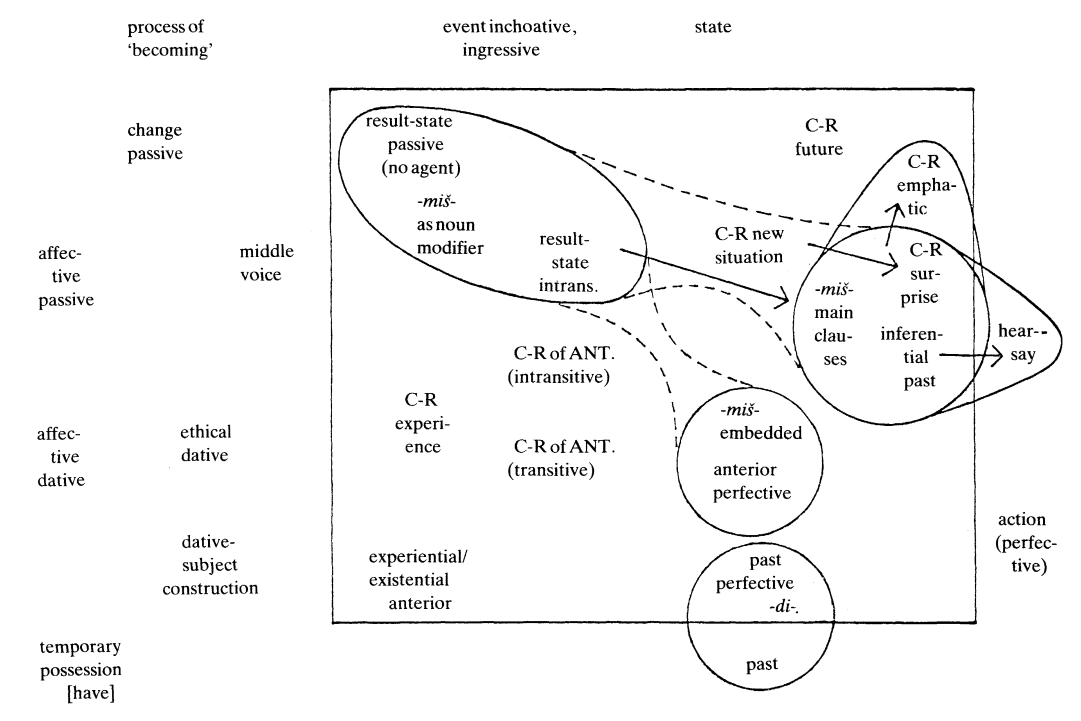
\includegraphics[scale=0.35]{images/turkmapanderson.png}}
\end{figure}

Согласно Айхенвальд, миративное <<расширение>> показателей косвенной засвидетельствованности часто восходит к инферентиву \citep[195]{aikhenvald2004}, связанному с моментом обнаружения ситуации. Для эвиденциальных перфектов это необязательно так. Напомним, что среди частных значений ТР имеется \textsc{недавнее прошедшее}, (или, по \citep{mccawley1971}, <<перфект горячих новостей>>), которое употребляется для передачи новой информации с оттенком удивления. Рисунок \ref{fig:semturk} представляет собой семантическую карту перфекта как типологической категории, на которой обведены употребления турецкого суффикса \textit{-mIš} \citep[234]{anderson1982}. Турецкий суффикс \textit{-mIš} чаще всего анализируется как показатель косвенно засвидетельствованного прошедшего, но он также может выражать и неожиданную ситуацию и восходит к перфектной форме \citep[188--190]{slobinaksukoc1982}. На карте Андерсона, миративное значение (C-R surprise) восходит именно к перфекту недавнего прошедшего (C-R new situation), якобы утраченному в турецком языке.
\par Ж. Лазар предлагал термин \textsc{медиатив} для форм, сочетающих эвиденциальную и миративную семантику (опираясь в основном на данные персидского и других иранских языков) \citep{lazard1956}. По мнению Лазара, значения инферентива, репортатива и миратива связывает более абстрактное значение отстранения, дистанцирования говорящего от передаваемой им самим информации. (Подобное рассуждение встречается в \citep{maisaktatevosov2007} в связи с данными цахурского языка нахско-дагестанской семьи.)

\begin{displayquote}
<<Speakers are somehow split into two persons, the one who speaks and the one who has heard or infers or perceives. This Operation distances them from their own discourse, whereas in neutral expression they adhere to their own discourse by virtue of the very laws of linguistic intercourse. The real value of the forms in question is this abstract distance, not any consideration of the nature of the source of the speaker's knowledge of the facts.>> \\
\citep[95]{lazard1999}
\end{displayquote}

Такое отстранение в турецком языке анализируется как <<прагматический эффект>> собственно эвиденциального значения в \citep[162--163]{slobinaksukoc1986}. Юхансон называет главной функцией таких форм в языках тюркской семьи <<to express the establishment of the event through the awareness of a conscious mind>> \citep[71]{johanson2000}. В зависимости от контекста, эта опосредованность наблюдателя приобретает самые разные конкретные прочтения. Стоит, однако, отметить, что употребление рассматриваемых форм в тюркских языках по мнению авторов при этом не связано с уверенностью говорящего в достоверности передаваемой информации, как в балканских славянских языках в анализе Фридмана.
\par Несмотря на то, что ярлык \textsc{эвиденциальность} многими считается не совсем подходящим для форм, типичных для эвиденциального пояса, большинство авторов (включая тех, кто предлагает альтернативные термины), причисляют эти формы к эвиденциальности как типологической категории, хотя и оговариваются, что значение этих форм на самом деле шире, чем простая оппозиция прямой и непрямой эвиденциальности. Судя по описаниям, полисемия, ассоциированная с этими формами, демонстрирует весьма разнообразные конфигурации в отдельных языках, а вопрос о том, как можно оценить их семантику в сравнительной перспективе, остается нерешенным. На фоне различных интерпретаций эвиденциальных перфектов в речи наиболее стабильным контекстом употребления нам представляется нарративный текст, поскольку значения ТР и миративности нехарактерны для описания последовательных событий и не усугубляют проблем теоретической интерпретации перфектоидов.
% Нужна ли тут ссылка? Я не знаю про источник, где было бы так сказано эксплицитно. Тем более текст, рассказан в перфекте может иметь оттенки фиктивности и сомнительности.
% Мне кажется, так нормально. Единственно, я не очень понимаю, почему в нарративе миративности не может быть - мне кажется, вполне естественно, нет?
Особенности употребления перфектоидов и форм косвенной засвидетельствованности в нарративе обсуждаются подробнее в разделе \ref{sec:intro3}.

% Самира, мне сейчас больше нравится, как вы сократили эту главу а в то, что от нее осталось, вплели ссылки на то, почему и где в дальнейшем исследовании это важно. Но именно в конце главы мне пока не хватает какого-то обобщения, финала - что будет в следующих главах, что мы узнали из этой главы, почему это важно для последующих глав. мне кажется, это отчасти ответило бы на претензии НРС и Дианы. Здесь было бы здорово в абзаце или в двух закруглить главу и направить читателя в нужном направлении. 
